\chapter{Representing Intent/Slot Concept with Natural Language Description}
\label{chap:sgd}

From early frame-driven dialog system GUS~\citep{bobrow1977gus} to
virtual assistants~(Alexa, Siri, and Google Assistant~\etal),
frame-based dialog state tracking has long been studied to meet
various challenges. In particular, how to support an ever-increasing
number of services and APIs spanning multiple domains has been a focal
point in recent years, evidenced by multi-domain dialog
modeling~\citep{budzianowski2018multiwoz,byrne2019taskmaster,
  shah-etal-2018-bootstrapping} and transferable dialog state tracking
to unseen intent/slots~\cite{mrkvsic2017neural,
  wu2019transferable, hosseini2020simple}.
\begin{figure}[!ht]
\centering
  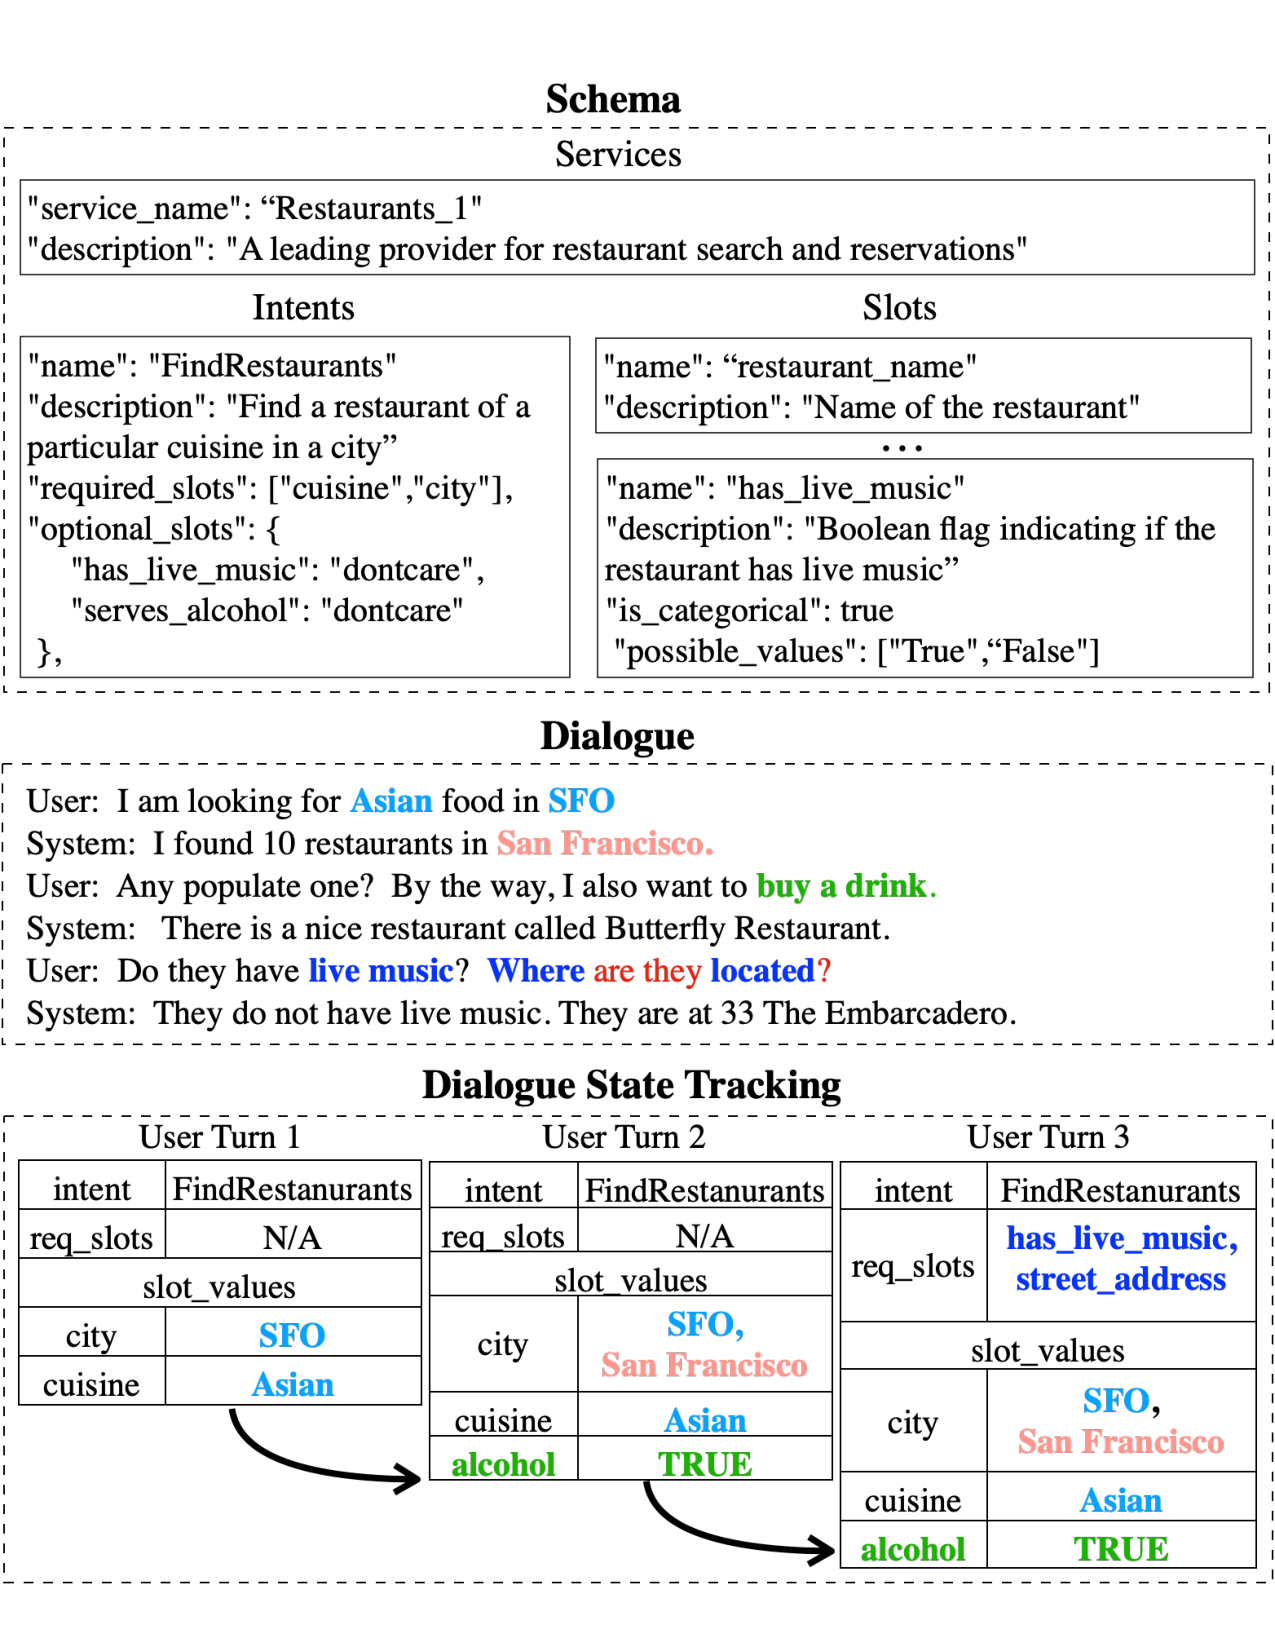
\includegraphics[width=0.90\textwidth]{schema-dst.pdf}
  \caption{\label{fig:schema-dst} An example dialog from Restaurant\_1 service, along with its service/intent/slot descriptions and dialog state representation.}
\end{figure}

Recently, \citet{rastogi2019towards} proposed a new paradigm called
schema-guided dialog for transferable dialog state tracking by using
natural language description to define a dynamic set of service
schemata. As shown in Figure \ref{fig:schema-dst}, the primary
motivation is that these descriptions can offer effective knowledge
sharing across different services, e.g., connecting semantically
similar concepts across heterogeneous APIs, thus allowing a unified
model to handle unseen services and APIs. With the publicly available
schema-guided dialog dataset~(\sgdst~henceforward) as a
testbed, they organized a state tracking shared task composed of four subtasks:
intent classfication~(\IC), requested slot identification~(\RSI),
categorical slot labeling~(\CSL), and noncategorical slot
labeling~(\NSL)~\cite{rastogi2020schema}. Many participants achieved
promising performance by exploiting the schema description for dialog
modeling, especially on unseen services.

Despite the novel approach and promising results, current
schema-guided dialog state tracking task only evaluates on a single
dataset with limited variation in schema definition. It is unknown how
this paradigm generalizes to other datasets and other different styles
of descriptions. In this paper, we focus our investigation on the
study of three aspects in schema-guided dialog state tracking:
\begin{inparaenum}[(1)]
\item schema encoding model architectures
\item supplementary training on intermediate tasks
\item various styles for schema description.
\end{inparaenum}
To make a more general discussion on
the schema-guided dialog state tracking, we perform extensive
empirical studies on both \sgdst~and~\multiwoz~datasets. In summary,
our contributions include:
\begin{itemize}
\item A comparative study
  on schema encoding architectures, suggesting a partial-attention
  encoder for good balance between inference speed and accuracy.
\item An experimental study of supplementary training on
  schema-guided dialog state tracking, via intermediate tasks
  including natural language inference and question answering.
\item An in-depth analysis of different schema description styles on a new
  suite of benchmarking datasets with
  variations in schema description for both \sgdst~and~\multiwoz.
\end{itemize}

\section{Schema-Guided Dialog State Tracking}
\label{sec:chanllenges-in-sgd}
%Before introducing the details on schema-guided dialog, we recap the
%general concepts in dialog state tracking by defining notations
%used in our paper. We use superscripts to denote the indices of
%dialog utterances, services, intents and slots, and subscripts for indices of tokens
%in a sequence. Suppose $U^{T}=[u^{1}, u^{2}, ... u^{T}]$ are a
%set of $T$ history utterances in the dialog,
%$V^{K}=[v^{1}, v^{2}...v^{K}]$ is a set of $K$ service schema
%supported by a dialog agent. For each service $v^{k}$, it consists
%of a set intent labels $I^{M}=[i^{1}, i^{2}...i^{M}]$, and slots
%labels $S^{N}=[s^{1}, s^{2}...s^{N}]$. A classic dialog state tracking
%task is to predict a dialog state frame $f^{t,k}$ at turn $t$ for each
%service $s^{k}$ given the dialog history $U$.
A classic dialog state tracker predicts a dialog state frame at each
user turn given the dialog history and predefined domain ontology. As
shown in Figure \ref{fig:schema-dst}, the key difference between
schema-guided dialog state tracking and the classic paradigm is the
newly added natural language descriptions.  In this section, we first
introduce the four subtasks and schema components in schema-guided
dialog state tracking, then we outline the research questions in our
paper.

\Paragraph{Subtasks} As shown in Figure \ref{fig:schema-dst}, the
dialog state for each service consists of 3 parts: {\it active
  intent}, {\it requested slots}, {\it user goals~(slot
  values)}. Without loss of generality, for both \sgdst and \multiwoz
datasets, we divide their slots into categorical and non-categorical
slots by following previous study on
dual-strategies~\cite{zhang2019find}. Thus to fill the dialog state
frame for each user turn, we solve four subtasks: intent
classification~(\IC), requested slot identification~(\RSI), categorical
slot labeling~(\CSL), and non-categorical slot labeling~(\NSL). All
subtasks require matching the current dialog history with candidate
schema descriptions for multiple times.

\Paragraph{Schema Components} Figure \ref{fig:schema-dst} shows three
main schema components: service, intent, slot. For each intent, the
schema also describes {\it optional} or {\it required} slots for
it. For each slot, there are flags indicating whether it is
categorical or not. {\it Categorical} means there is a set of
predefined candidate values~(Boolean, numeric or text). For instance,
{\it has\_live\_music} in Figure~\ref{fig:schema-dst} is a categorical
slot with Boolean values. {\it Non-categorical}, on the other hand,
means the slot values are filled from the string spans in the dialog
history.

\Paragraph{New Questions} These added schema descriptions pose
the following three new questions. We discuss each of them in the
following sections.
\\
\setlength{\fboxsep}{1.5pt}
\fbox{\small\parbox{0.90\textwidth}{
\begin{enumerate}[label=Q\arabic*.]
\item How should dialogue and schema be encoded? \S\ref{sec:models}
\item How do different supplementary trainings impact each subtask? \S\ref{sec:sup-training}
\item How do different description styles impact the state tracking performance? \S\ref{sec:abl-desc}
\end{enumerate}
}}

%%% Local Variables:
%%% mode: latex
%%% TeX-master: "../../thesis-main.ltx"
%%% End:


\section{Related Work}
\label{sec:sgd:related-work}
Our work is related to three lines of research: multisentence
encoding, multidomain and transferable dialogue state
tracking. However, our focus is on the comparative study of different
encoder architectures, supplementary training, and schema
description style variation. Thus we adopt existing strategies from
multidomain dialogue state tracking.

\subsection{Multisentence Encoder Strategies}
\label{ssec:sgd:multi-encoder}
Similar to the recent study on encoders for response selection and
article search tasks~\citet{humeau2019poly}, we also conduct our
comparative study on the two typical architectures
\CE~\citep{bordes2014open, lowe2015ubuntu} and
\DE~\citep{wu2017sequential,yang2018response}. However, they only focus
on sentence-level matching tasks. All subtasks in our case require
sentence-level matching between dialogue context and each schema, while
the noncategorical slot filling task also needs to produce a sequence
of token-level representation for span detection. Hence, we study
multisentence encoding for both sentence-level and token-level
tasks. Moreover, to share the schema encoding across subtasks and
turns, we also introduce a simple \FE by caching schema token
embeddings in~\autoref{ssec:encoder-arch}, which improves efficiency
without sacrificing much accuracy.
%% YZ: not sure how the following point fits in here
%Beside that, rather
%than a provided set of candidate sentences to match in sentence
%selction tasks, we also study different compositions of schema
%components as candidates in~\autoref{sssec:com-desc}, e.g. compositions
%of service, intent, slot descriptions.

\subsection{Multidomain Dialogue State Tracking}
\label{ssec:sgd:multidomain}
Recent research on multidomain dialogue system have been largely driven
by the release of large-scale multidomain dialogue datasets, such as
MultiWOZ~\citep{budzianowski2018multiwoz},
M2M~\citep{shah-etal-2018-bootstrapping}, accompanied by studies on key
issues such as in/cross-domain carry-over~\citep{ kim2019efficient}. In
this paper, our goal is to understanding the design choice for schema
descriptions in dialogue state tracking.  Thus we simply follow the
in-domain cross-over strategies used in {\bf
  TRADE}~\citep{wu2019transferable}. Additionally, explicit
cross-domain carryover~\citep{naik2018contextual} is difficult to
generalize to new services and unknown carryover links. We use longer
dialogue history to inform the model on the dialogue in the previous
service. This simplified strategy does impact our model performance
negatively in comparison to a well-designed dialogue state tracking
model on seen domains. However, it helps reduce the complexity of
matching extra slot descriptions for cross-service carryover. We leave
the further discussion for future work.

\subsection{Transferable Dialogue State Tracking}
\label{ssec:sgd:transfer-dialogue}
Another line of research focuses on how to build a transferable dialogue
system that is easily scalable to newly added intents and slots. This
covers diverse topics including, \eg, resolving lexical/morphological
variabilities by symbolic delexicalization-based
methods~\citep{henderson2014word, williams2016dialog}, neural belief
tracking~\citep{mrkvsic2017neural}, generative dialogue state
tracking~\citep{peng2020soloist, hosseini2020simple}, modeling DST as a
question answering task~\citep{zhang2019find, lee2019sumbt,
  gao2020machine, gao2019dialog}. Our work is similar with the last
class. However, we further investigate whether the DST can benefit
from NLP tasks other than question answering. Furthermore, without
rich description for the service/intent/slot in the schema, previous
works mainly focus on simple format on question answering scenarios,
such as domain-slot-type compounded names~(\eg, ``{\it
  restaurant-food}"), or simple question template ``{\it What is the
  value for {\bf slot i}?}". We incorporate different description
styles into a comparative discussion in~\autoref{ssec:desc-styles}.

%%% Local Variables:
%%% mode: latex
%%% TeX-master: "../../dissertation-main.ltx"
%%% End:


\section{Datasets and Model Setup}
\label{sec:sgd:datasets}

\begin{table}[!t]
\caption{\label{tbl:sgd:datasets} Summary of characteristics of \sgdst \multiwoz datasets, in domain diversity, function overlap, data collecting methods.}
\begin{center}{
\setlength{\tabcolsep}{3pt}
\begin{tabular}{l|ccccc|c|c}
\toprule
\hline
\multirow{2}{*}{Datasets}                   & \multirow{2}{*}{Splits} & \multirow{2}{*}{Dialog} & Domains  & Zero-shot & Zero-shot & Function & Collecting             \\
                                            &                         &                         & (Services) & Domains   & Services  & Overlapp & Method                 \\ \hline
\multirow{3}{*}{ \sgdst}                    & Train                   & 16142                   & 16(26)   & -         & -         & Across/  & \multirow{3}{*}{ M2M}  \\
                                            & Dev                     & 2482                    & 16(17)   & 1         & 8         & Within   &                        \\
                                            & Test                    & 4201                    & 18(21)   & 3         & 11        & Domain   &                        \\ \hline
\multirow{3}{*}{\parbox[c]{2cm}{\multiwoz}} & Train                   & 9617                    & 3(3)     & -         & -         & Across   & \multirow{3}{*}{ H2H } \\
                                            & Dev                     & 2455                    & 5(5)     & 2         & 2         & Domain   &                        \\
                                            & Test                    & 2969                    & 8(8)     & 5         & 5         &          &                        \\ \hline
\bottomrule
\end{tabular}}
\end{center}
\end{table}

To the best of our knowledge, at the time of our study, \sgdst~and
\multiwoz~are the only two publicly available corpus for schema-guided
dialog study. We choose both of them for our study. In this section,
we first introduce these two representative datasets, then we discuss
the generalizibility in domain diversity, function overlapping, data
collecting methods.

\subsection{Schema-Guided Dialog Dataset}
\label{ssec:sgd:schema-dataset}
\sgdst
dataset~\footnote{\url{https://github.com/google-research-datasets/dstc8-schema-guided-dialogue}}
is especially designed as a test-bed for schema-guided dialog, which
contains well-designed heterogeneous APIs with overlapping
functionalities between services~\cite{rastogi2019towards}. In
DSTC8~\cite{rastogi2020schema}, \sgdst~was introduced as the standard
benchmark dataset for schema-guided dialog research. \sgdst~covers 20
domains, 88 intents, 365 slots.\footnote{Please refer to~\citet{rastogi2019towards} for more details.} However, previous research are mainly
conducted based on this single dataset and the provided single
description style. In this paper, we further extended this dataset
with other benchmarking description styles as shown in~\autoref{sec:sgd:abl-desc}, and then we perform both homogenous and
hetergenous evalution on it.

\subsection{Remixed MultiWOZ 2.2 Dataset}
\label{ssec:sgd:multiwoz-dataset}

To eliminate potential bias from the above single \sgdst~dataset, we
further add \multiwoz~\cite{zang-etal-2020-multiwoz} to our study.

To evaluate performance on seen/unseen services with MultiWOZ, we
remix the \multiwoz dataset to include as seen services dialogs
related to \textit{restaurant}, \textit{attraction} and \textit{train}
during training, and eliminate slots from other domains/services from
training split.  For dev, we add two new domains {\it hotel} and {\it
  taxi} as unseen services. For test, we add all remaining domains as
unseen, including those that have minimum overlap with seen services,
such as {\it hospital}, {\it police}, {\it bus}. The statistics are as
shown in Table \ref{tbl:multiwoz-remix}.

\begin{table}[t]
\caption{\label{tbl:multiwoz-remix} The total number of dialogs and
  turns related to each domain in train, dev and test split of MultiWOZ.}
\begin{center}{
\setlength{\tabcolsep}{3pt}
\begin{tabular}{ccccccc}
 \toprule

\multirow{2}{*}{Domain } & \multicolumn{6}{c}{\#dialogs/\#turns}                                                \\ \cmidrule{2-7}
                         & \multicolumn{2}{c}{ train } & \multicolumn{2}{c}{ dev } & \multicolumn{2}{c}{ test } \\ \hline
restaurant               & 3900                        & 37953                     & 458 & 6979 & 451 & 7104    \\
attraction               & 2716                        & 28632                     & 405 & 6198 & 400 & 6290    \\
train                    & 3001                        & 29646                     & 481 & 5897 & 491 & 6150    \\
hotel                    & 0                           & 0                         & 737 & 8509 & 718 & 7911    \\
taxi                     & 0                           & 0                         & 374 & 2692 & 364 & 2659    \\
hospital                 & 0                           & 0                         & 0   & 0    & 287 & 766     \\
police                   & 0                           & 0                         & 0   & 0    & 252 & 475     \\
bus                      & 0                           & 0                         & 0   & 0    & 6   & 132     \\
 \bottomrule
\end{tabular}}
\end{center}
\end{table}

%Multi-Domain Wizard-of-Oz dataset was first introduced
%in~\citet{budzianowski2018multiwoz}. With the large-scale fully
%annotated dialog data, it has pushed forward the research on
%multi-domain task-oriendted
%dialog~\cite{kim2019efficient,wu2019transferable,
%  hosseini2020simple}. Then, 
Among various extended versions for MultiWOZ
dataset~\cite[2.0-2.3,][]{budzianowski2018multiwoz,
  eric2020multiwoz,zang-etal-2020-multiwoz,han2020multiwoz} , besides
rectifying the annotation errors, \multiwoz ~also introduced the
schema-guided annotations, which covers 8 domains, 19 intents, 36
slots.  To evaluate performance on seen/unseen services with MultiWOZ,
we remix the \multiwoz~dataset to include as seen services dialogs
related to \kw{restaurant}, \kw{attraction} and \kw{train}
during training, and eliminate slots from other domains/services from
training split.  For dev, we add two new domains \kw{hotel} and \kw{taxi} as unseen services. For test, we add all remaining domains as
unseen, including those that have minimum overlap with seen services,
such as \kw{hospital}, \kw{police}, \kw{bus}. The statistics of
data splits are shown in
~\autoref{tbl:multiwoz-remix}. Note that this data split
is different from the previous work on zero-shot MultiWOZ DST which
takes a leave-one-out approach in~\citet{wu2019transferable}. By
remixing the data in the way described above, we can evaluate the
zero-shot performance on MultiWOZ in a way largely compatible with
\sgdst.

\subsection{Discussion on Datasets}
\label{ssec:sgd:discussion-datasets}

First, the two datasets cover diverse domains. \multiwoz~covers
various possible dialogue scenarios ranging from requesting basic
information about attractions through booking a hotel room or
travelling between cities. While \sgdst~covers more domains, such as
`Payments', `Calender', `DoctorServices' and so on.

Second, they include different levels of overlapping
functionalities. \sgdst~allows frequent function overlapping between
multiple services, within the same domain~(\eg, BookOneWayTicket
v.s. BookRoundTripTicket), or across different domains~(BusTicket
v.s. TrainTicket). However, the overlapping in \multiwoz~only exists
across different domains, \eg, `destination', `leaveat' slots for
Taxi and Bus services, `pricerange', `bookday' for Restaurant and
Hotel services.

Third, they are collected by two different approaches which are
commonly used in dialog collecting. \sgdst~is firstly collected by
machine-to-machine self-play~\cite[M2M,][]{shah2018building} with
dialog flows as seeds, then paraphrased by crowd-workers. While
\multiwoz~are human-to-human
dialogs~\cite[H2H,][]{kelley1984iterative}, which are collected with
the Wizard-of-Oz approach.

We summarize the above discussion in~\autoref{tbl:sgd:datasets}.  We
believe that results derived from these two representative datasets can
guide future research in schema guided dialogue.


\subsection{Experiment Setup}
\label{ssec:sgd:exp-setup}
All models are based on BERT-base-cased model with 2 V100 GPUs~(with
16GB GPU RAM each). We train each models for maximum 10 epoch, by
using AdamW to schedule the learning rate with a warm-up portion of
0.1. During training, we evaluate checkpoints per 3000 steps on dev
splits, and select the model with best performance on dev split on all
seen and unseen services. In our experiments, our model achieves the
best performance on around 2-4 epochs on \IC, \RSI. and \CSL, while
\NSL needs 5-8 epochs to get the best performance. For all subtasks, as
we model all of them as sentence pair encoding during training, we use
batch size as 16 for each GPU, and gradient accumulate for 8 steps, in
total 256 batch size on 2 GPUs.

%%% Local Variables:
%%% mode: latex
%%% TeX-master: "../../dissertation-main.ltx"
%%% End:


\section{Dialog \& Schema Representation and Inference~(Q1)}
\label{sec:sgd:models}
In this section, we focus on the model architecture for matching
dialog history with schema descriptions using pretrained
BERT~\cite{devlin2019bert}~\footnote{We use BERT-base-cased for all
  main experiments. Other pretrained language models can be easily adapted to our study}. To support four subtasks,
we first extend \DE and \CE~to support both sentence-level matching and token-level
prediction. Then we propose an additional \FE strategy to get faster
inference without sacrificing much accuracy. We summarize different
architectures in Figure \ref{fig:encoders}. Then we show the
classification head and results for each subtask.

\begin{figure}[!t]
\centering
  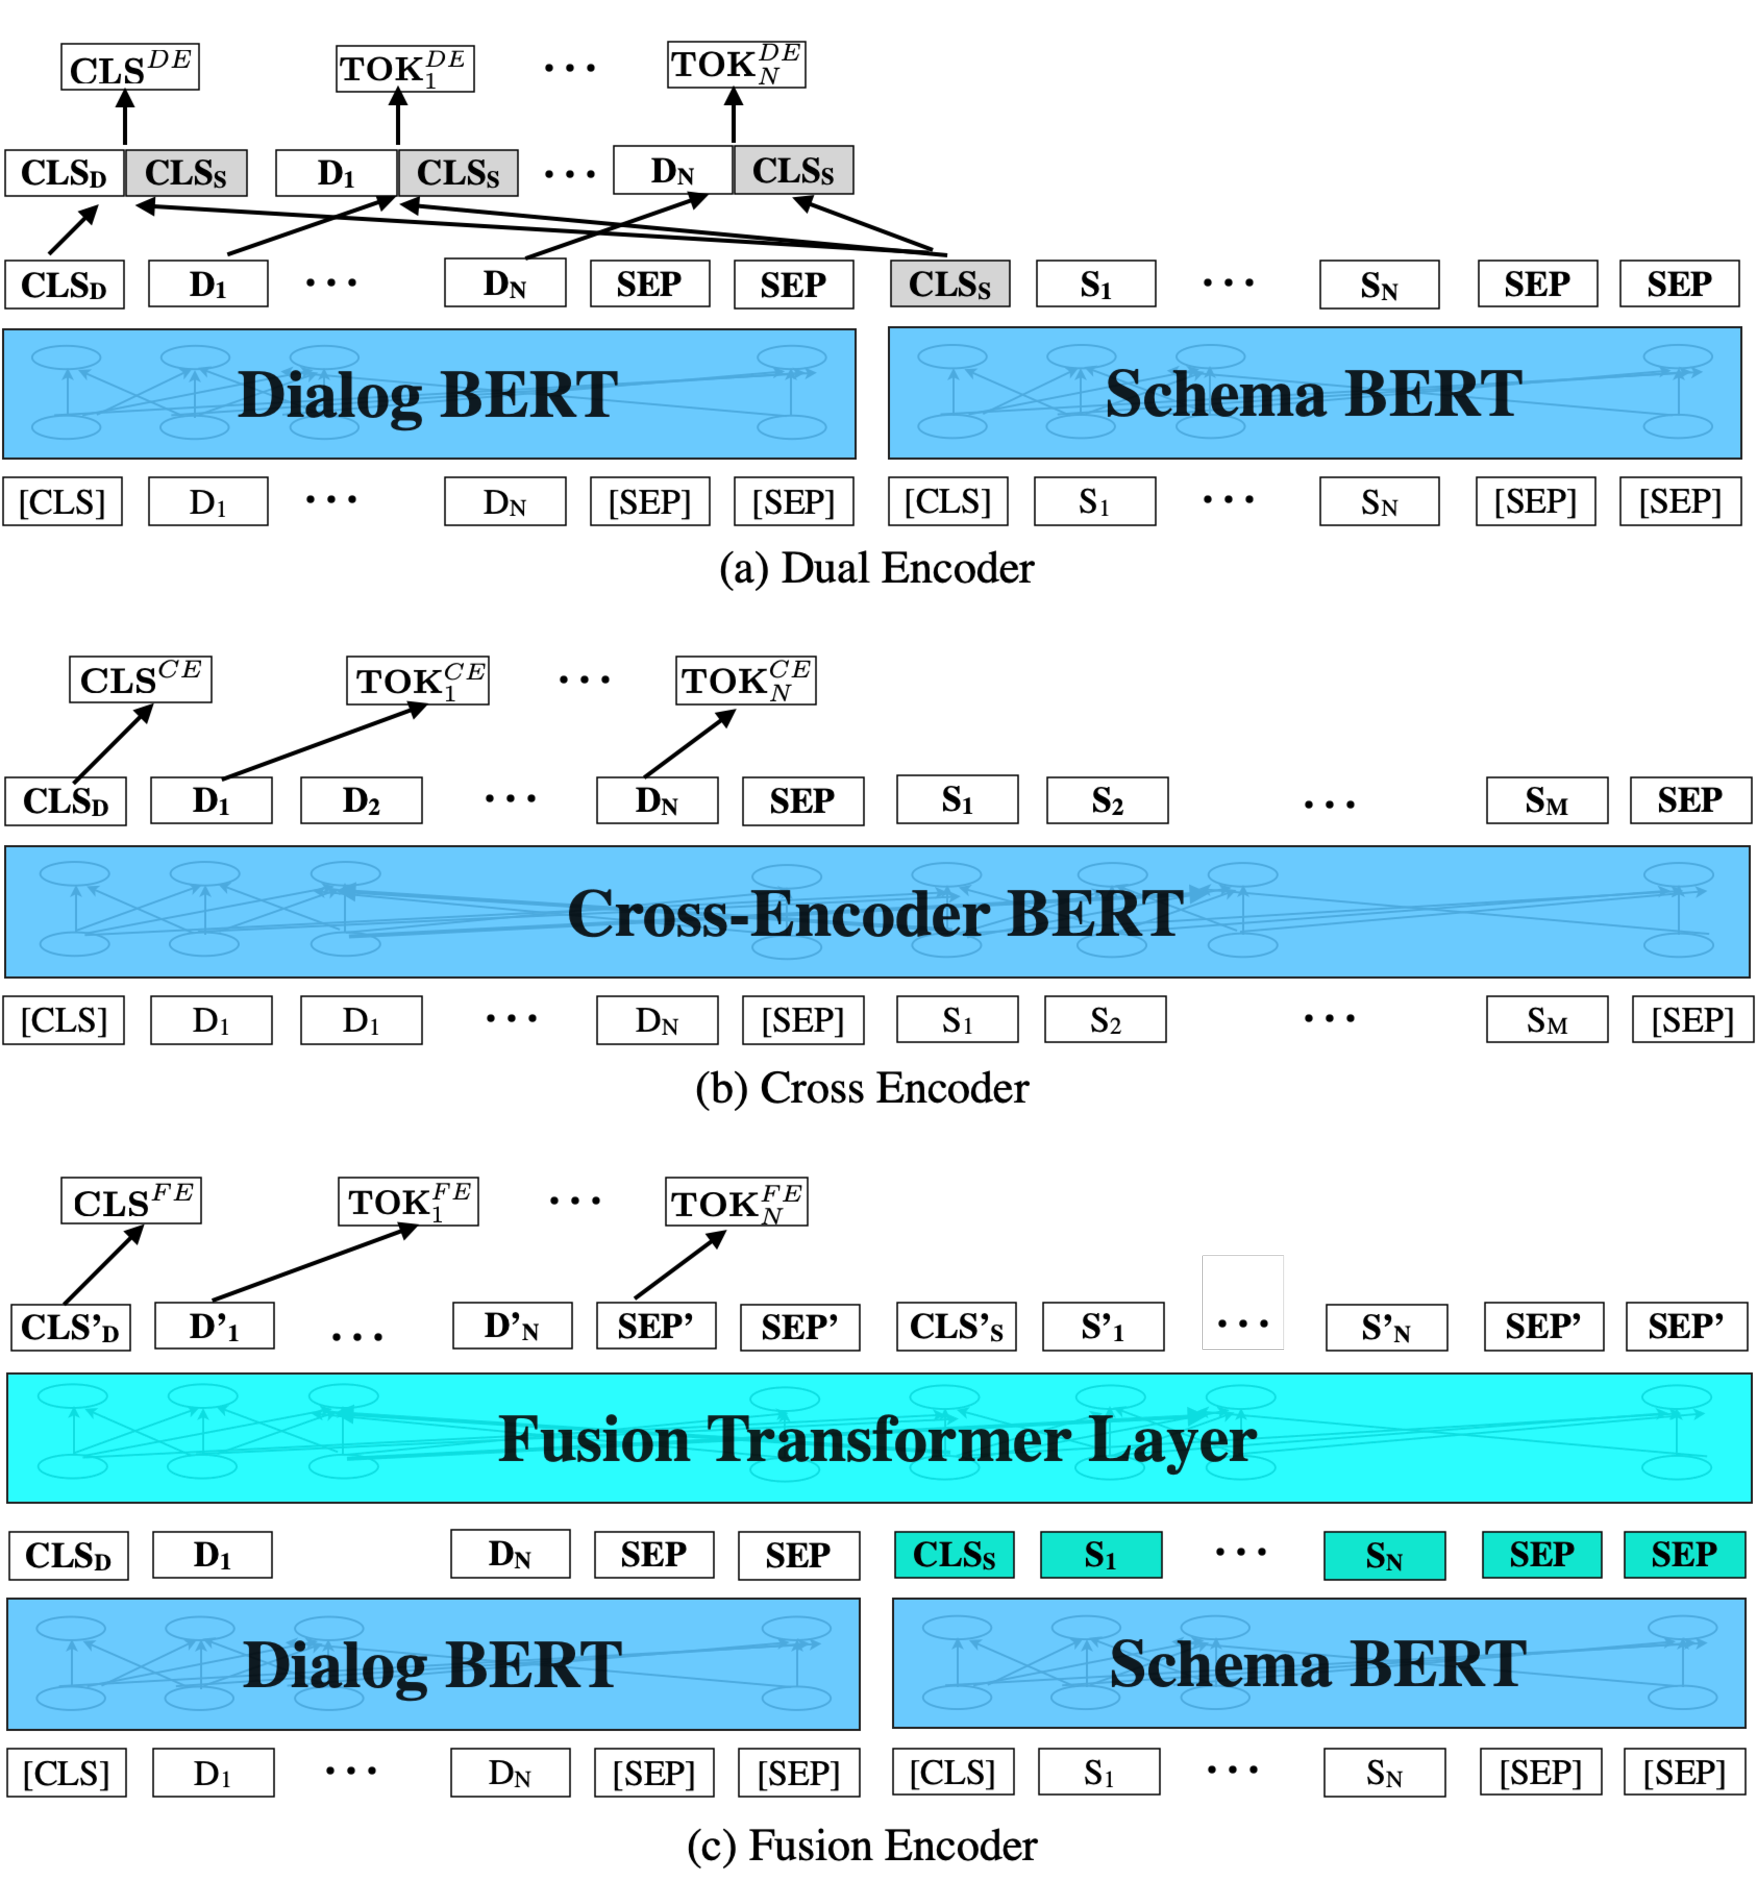
\includegraphics[width=0.90\textwidth]{all-encoders.pdf}
  \caption{\label{fig:encoders} Dual-Encoder, Cross-Encoder and Fusion Encoder, shaded block will be cached during training}
\end{figure}

\subsection{Encoder Architectures}
\label{ssec:encoder-arch}
\Paragraph{Dual-Encoder} It consists of two separate BERTs to encode
dialog history and schema description respectively, as
Figure~\ref{fig:encoders}~(a). We follow the setting in the official
baseline provided by DSTC8 Track4~\cite{rastogi2020schema}. We first
use a fixed BERT to encode the schema description once and cached the
encoded schema $\CLS_{S}$. Then for sentence-level representation, we
concatenate dialog history representation $\CLS_{D}$ and candidate
schema representation $\CLS_{S}$ as the whole sentence-level
representation for the pair, denoted as~${\CLS^{DE}}$.  For
token-level representation, we concatenate the candidate schema
$\CLS_{S}$ with each token embedding in the dialog history, denoted
as~${\TOK^{DE}}$.\footnote{A schema-aware dialog token embedding can
  also be computed by attention or other method for span-based
  detection tasks~\cite{humeau2019poly, noroozi2020fast}} Because
the candidate schema embeddings are encoded independently from the
dialog context, they can be pre-computed once and cached for fast
inference.

\Paragraph{Cross-Encoder} Another popular architecture as
Figure~\ref{fig:encoders}~(b) is \CE, which concatenates the dialog
and schema as a single input, and encodes jointly with a single
self-attentive encoder spanning over the two segments.  When using
BERT to encode the concatenated sentence pair, it performs
full~(cross) self-attention in every transformer layers, thus offer
rich interaction between the dialog and schema. BERT naturally
produces a summarized representation with [CLS]
embedding~${\CLS^{CE}}$ and each schema-attended dialog token
embeddings~${\TOK^{CE}}$. Since the dialog and schema encoding always
depend on each other, it requires recomputing dialog and schema
encoding for multiple times, thus much slower in inference.
%
%\subsubsection{Poly-Encoder}
%\label{sssec:poly-encoder}
%Poly-Encoder~\citet{humeau2019poly} was proposed to response selection
%and article retrieval tasks, where a pair of context and candidate
%sentences need to be encoded. Extending to our schema-guided dialog
%task, the pair of text are dialog context and schema
%descriptions. Poly-Encoder seperately encode the schemas, thus can
%precompute and cache all the schema embedding, which is adopted from
%the Dual-Encoder, thus efficient for training and inference; Then for
%context dialog encoding, Poly-Encoder borrow the cross attention
%ability from Cross-Encoder, it first predicts $m$ different
%representation vector for dialog context rather than a single vector
%in Dual-Encoder, then it attend over them using the precomputed single
%schema as a query, finally sum up all the weighted dialog context as
%schema-aware dialog representation.

\Paragraph{Fusion-Encoder} In Figure~\ref{fig:encoders}~(c), similar
to \DE, \FE also encodes the schema independently with a fixed BERT
and finetuning another BERT for dialog encoding. However, instead of
caching a single [CLS] vector for schema representation, it caches {\bf all
token representation} for the schema including the [CLS] token. What's
more, to integrate the sequences dialog token representation with
schema token representation, an extra stack of transformer layers are
added on top to allow token-level fusion via self-attention, similar
to \CE. The top transformer layers will produce embeddings for each
token~${\TOK^{FE}}$ including a schema-attended
~${\CLS^{FE}}$ of the input [CLS] from the dialog
history. With cached schema token-level representations, it can
efficiently produce schema-aware sentence- and token-level
representation for each dialog-schema pairs.

\subsection{Model Overview}
\label{ssec:models-overview}
All the above 3 encoders will produce both sentence- and token-level
representations for a given sentence pair. In this section,
we abstract them as two representations~\CLS~and~\TOK, and present the
universal classification heads to make decisions for each subtask.
%Especially, slots from previous dialog state can be carried over to
%the next dialog state, cross the same or different dialog state. For
%example, the hotel name in the hotel-booking service can be carried
%over to the detination in the taxi-service, while the amount in
%``MakePayment" cannot be carried to ``RequestPayment". The strategies
%for those common dialog state tracking strategies such as two-stage,
%overwriting memory, end2end has been widely studied in previous work.

\Paragraph{Active Intent} To decide the intent for current dialog
turn, we match current dialog history $D$ with each intent
descriptions $I_{0}...I_{k}$. For each dialog-intent pair $(D,I_{k})$,
we project the final sentence-level \CLS~representation to a single
number $P_{I_{k}}^{active}$ with a linear layer follows a sigmoid
function. We predict \textit{"NONE"} if the $P_{I_{k}}^{active}$ of
all intents are less than a threshold 0.5, which means no intent is
active. Otherwise, we predict the intent with largest
$P_{I_{k}}^{active}$. We predict the intent for each turn
independently without considering the prediction on previous turns.

\Paragraph{Requested Slot} As in Figure~\ref{fig:schema-dst},
mulitple requested slots can exist in a single turn. We use the
same strategy as in active intent prediction to predict a number
$P_{req}^{active}$. However, to support the multiple requested slots
prediction. We predict all the requested slots with
$P_{req}^{active} > 0.5$.

\Paragraph{Categorical Slot} Categorical slots have a set of candidate
values. We cannot predict unseen values via n-way
classification. Instead, we do binary classification on each candidate
value. Besides, rather than directly matching with values, we also
need to check that whether the corresponding slot has been
activated. For \CE and \FE, we use typical two-stage state tracking to
incrementally build the state:
\begin{inparaenum}[{\bf Step} 1.]
\item Using ~$\mathbf{CLS}$ to predict the slot status as
  \textit{none}, \textit{dontcare} or \textit{active}. When the status is
  \textit{active}, we use the predicted slot value; Otherwise, it
  will be assigned to \textit{dontcare} meaning no user preference for this
  slot, or \textit{none} meaning no value update for the slot in current turn;
\item If Step 1 is \textit{active}, we match the dialog
  history with each value and select the most related value by ranking. We train on cross entropy loss.
\end{inparaenum}
Two-stage strategy is efficient for \DE and \FE, where cached schema
can be reused, and get efficiently ranked globally in a single
batch. However, it is not scalable for \CE, especially for large
number of candidate values in MultiWOZ dataset. Hence, during
training, we only use a binary cross-entropy for each single value and
postpone the ranking only to the inference time.

\Paragraph{Noncategorical Slot} The slot status prediction for
noncategorical slot use the same two-stage strategy. Besides that, we
use the token representation of dialog history ~$\mathbf{TOK}$ to
compute two softmax scores $f^{i}_{start}$ and $f^{i}_{end}$ for each
token $i$, to represent the score of predicting the token as start and
end position respectively. Finally, we find the valid span with
maximum sum of the start and end scores.

%% YZ: please check the correctness of the noncat slot prediction head description^^
\subsection{Experiments on Encoder Comparison}
\label{ssec:encoder-results}
To fairly compare all three models, we follow the same schema input
setting as in Table \ref{tbl:schema-seq}. We trained separate models
for \sgdst~and the remixed MultiWOZ datasets for all the experiments
in our papers\footnote{Appendix~\ref{ssec:exp-setup} shows the
  detailed experiment setup}. Because there are very few intent and
requested slots in \multiwoz~dataset, we ignore the intent and
requested slots tasks for \multiwoz~in our paper.


\begin{table}[!t]
\begin{center}{\small
\setlength{\tabcolsep}{3pt}
\begin{tabular}{l|c}
  \toprule
\hline
Intent & service description, intent description \\
Req    & service description, slot description   \\
Cat    & slot description, cat value             \\
NonCat & service description, slot description   \\
\hline
  \bottomrule
\end{tabular}}
\end{center}
\caption{\label{tbl:schema-seq} Schema description input used for
  different tasks to compare \DE, \CE, and \FE. In the
  appendix~\ref{ssec:com-desc}, we also studies other compositions of
description input. We found that service description will not help for
\IC, \RSI and~\CSL tasks, while the impact on \NSL~task also varies
from \sgdst~and~\multiwoz~dataset.}
\end{table}

%Previous paper on zero-shot
%MultiWOZ conduct zero-shot experiments on 5 domains. Then they train
%on four domains and evaluate on one heldout domain. Thus 5 different
%models needs to be trained to evaluate the zero-shot performance. To
%make a universal comparision with SG-DST dataset, we remix the
%MultiWOZ 2.2 dataset to have unseen domains in the both dev and
%test. In training split, we use all the dialogs related to restaunt,
%attration and train, and remove those slots belong to unseen
%domain. Then for dev, we add two new domains {\it hotel} and {\it taxi}
%domains, while for test, we add all remaining unseen domains,
%epecially, we also involved new domains that are don't have much
%overlapping with seen domains, such as {\it hospital}, {\it police},
%{\it bus}. By reorgianing the dataset as above, we offer a new way to
%evaluate the zero-shot performance on multiwoz with less effort.
%More The main statistics as shown in Table \ref{multiwoz-resplit}

\Paragraph{Results} As shown in Table~\ref{tbl:sgd-modeling-results},
\CE~performs the best over all subtasks. Our \FE with partial
attention outperforms the \DE by a large margin, epsecially on
categorical and noncategorical slots predictions. Additionally, on
seen services, we found that \DE and \FE can perform as good as \CE on
\IC and \RSI tasks. However, they cannot generalize well on unseen
services as \CE. %However, their
%model are specially optimized for SG-DST dataset on DSTC8 contest,
%including using adopting dialog state from system turn, hand-crafted
%features, dev set, data augmentation, ensemble methods, thus the
%performance are not comparable.

\begin{table}[!t]
\begin{center}{
\setlength{\tabcolsep}{4pt}
\begin{tabular}{l|ccccc|ccc}
  \toprule
  \hline
  \multirow{3}{*}{Method/Task} & \multicolumn{5}{c}{\sgdst} & \multicolumn{3}{c}{\multiwoz}                                                                                      \\ \hline
                               & Acc                        & F1          & \multicolumn{3}{c|}{Joint Acc} & \multicolumn{3}{c}{Joint Acc}                                       \\
                               & Intent                     & Req         & Cat                            & NonCat      & All         & Cat         & NonCat      & All         \\ \hline
  \multicolumn{9}{c}{{\bf Seen Services}}                                                                                                                                        \\ \hline
  % SOTA                       & 95.71                      & 99.36       & N.A                            & N.A         & 92.41       & N.A         & N.A         & N.A         \\ \hline
  Dual-Encoder                 & 94.51                      & 99.62       & 87.92                          & 47.77       & 43.20       & 79.20       & 79.34       & 65.64       \\
  Fusion-Encoder               & 94.90                      & {\bf 99.69} & 88.94                          & 48.78       & 58.52       & 81.37       & 80.58       & 67.43       \\
  Cross-Encoder                & {\bf 95.55}                & 99.59       & {\bf 93.68}                    & {\bf 91.85} & {\bf 87.58} & {\bf 85.99} & {\bf 81.02} & {\bf 71.93} \\ \hline
  \multicolumn{9}{c}{{\bf Unseen Services}}                                                                                                                                      \\ \hline
  % SOTA                       & 94.52                      & 98.17       & N.A                            & N.A         & 84.56       & N.A         & N.A         & N.A         \\ \hline
  Dual-Encoder                 & 89.73                      & 95.20       & 42.44                          & 31.62       & 19.51       & 56.92       & 50.82       & 31.83       \\
  Fusion-Encoder               & 90.47                      & 95.95       & 48.79                          & 35.91       & 22.85       & 57.01       & 52.23       & 33.64       \\
  Cross-Encoder                & {\bf 93.84}                & {\bf 98.26} & {\bf 71.55}                    & {\bf 74.13} & {\bf 54.54} & {\bf 59.85} & {\bf 59.62} & {\bf 38.46} \\ \hline
  \bottomrule
\end{tabular}}
\end{center}
\caption{\label{tbl:sgd-modeling-results} Test set results on \sgdst and \multiwoz. The
  \DE model is a re-implementation of official DSTC8
  baseline from \citet{rastogi2019towards}. Other models are
  trained with the architecture described in our paper.}
\end{table}

\Paragraph{Inference Speed} To test the inference speed, we conduct
all the experiments with a maximum affordable batch size to fully
exploit 2 V100 GPUs (with 16GB GPU RAM each). During training, we log
the inference time of each evaluation on dev set. Both \DE and \FE can
do joint inference across 4 subtasks to obtain an integral dialog
state for a dialog turn example. \DE achieves the highest inference
speed of {\bf 603.35} examples per GPU second, because the encoding
for dialog and schema are fully separated. A dialog only needed to be
encoded for once during the inference of a dialog state example while
the schema are precomputed once. However, for \CE, to predict a dialog
state for a single turn, it need to encode more than 300 sentence
pairs in a batch, thus only processes {\bf 4.75} examples per GPU
second. \FE performs one time encoding on dialog history, but it needs
to jointly encode the same amount of dialog-schema pair ws \CE,
instead, however, with a two-layer transformer encoder. Overall it
achieves {\bf 10.54} examples per GPU second, which is {\bf 2.2x}
faster than \CE. With regarding to the accuracy in
Table~\ref{tbl:sgd-modeling-results}, \FE~performs much better than
\DE, especially on unseen services.
% More details of the performance on each subtasks are shown in Table \ref{tbl:encoder-speed}.

%%% Local Variables:
%%% mode: latex
%%% TeX-master: "../../thesis-main.ltx"
%%% End:


\section{Supplementary Training~(Q2)}
\label{sec:sgd:sup-training}
Besides the pretrain-fintune framework used in \S\ref{sec:sgd:models},
\citet{phang2018sentence} propose to add a supplementary training
phase on an intermediate task after the pretraining, but before
finetuning on target task. It shows significant improvement on the
target tasks. Moreover, large amount pretrained and finetuned
transformer-based models are publicly accessible, and well-organized
in model hubs for sharing, training and testing\footnote{e.g.,
  Huggingface(\url{https://huggingface.co/models}) and
  ParlAL(\url{https://parl.ai/docs/zoo.html}), etc.}.  Given the new
task of schema-guided dialog state tracking, in this section, we study
our four subtasks with different intermediate tasks for supplementary
training. However, how to choose those intermediate tasks is a
challenge problem. Our inductive biases on choosing intermediate tasks
are: \textit{Intermediate tasks that sharing similar structures with
  downsteam tasks may help the supplementary training.}  Hence, for
natural language description modelling, we will first show the
similarity between our proposed \textbf{Natural Language inference}
and \textbf{Question Ansering} with our four subtasks, then analyze
the results on how they performed.

\subsection{Intermediate Tasks}
\label{ssec:intermediate-tasks}
As described in \S~\ref{ssec:models-overview}, all our 4
subtasks take a pair of dialog and schema description as input, and
predict with the summerized sentence-pair~\CLS~representation. While
\NSL~also requires span-based detection such as question
answering. Hence, they share the similar problem structure with the
following sentence-pair encoding tasks.

\Paragraph{Natural Language Inference} Given a hypothesis/premise
sentence pair, natural language inference is a task to determine
whether a hypothesis is entailed, contradicted or neutral given
that premise.

\Paragraph{Question Answering} Given a passage/question pairs, the
task is to extract the span-based answer in the passage.

Hence, when finetuning BERT on our subtaks, instead of directly using
the originally pretrained BERT, we use the BERT
finetuned on the above two tasks for further finetuning.  Due to better
peformance of \CE in \S\ref{ssec:models-overview}, we directly use the finetuned
\CE~version of BERT models on SNLI and SQuAD2.0 dataset from
Huggingface model hub. We add extra speaker tokens [user:] and
[system:] into the vocabulary for encoding the multi-turn dialog
histories.
%
%\Paragraph{Response Selection} Given a dialog history and a set of
%candidate response, the task is to select the best response follow the
%dialog hisotry. We didn't find any public BERT Cross-encoder model
%finetuned on this task. Hence, we finetuned a cross-encoder model on
%ConvAI2 dataset with code provided in ParlAI.

\subsection{Results on Supplementary Training}
\label{ssec:sgd:results-secondary}

\begin{table}[!t]
\begin{center}{
\setlength{\tabcolsep}{2pt}
\begin{tabular}{c|ccc|ccc|ccc|ccc}
  \toprule
  \hline
                       & \multicolumn{12}{c}{ \sgdst } \\ \cline{2-13}
                       & \multicolumn{3}{c|}{ intent }  & \multicolumn{3}{c|}{ req } & \multicolumn{3}{c|}{ cat } & \multicolumn{3}{c}{ noncat } \\ \cline{2-13}
                       & all                            & seen                       & unseen                     & all                           & seen                       & unseen & all   & seen  & unseen & all        & seen  & unseen     \\ \hline
  $\Delta_{\textbf{SNLI}}$  & {\bf +0.51}                    & +0.02                      & {\bf +0.68}                & -0.19                         & +0.38                      & -0.38  & -1.63 & -2.87 & -1.23  & -4.7       & -0.1  & -6.25      \\ \hline
  $\Delta_{\textbf{SQuAD}}$ & -1.81                          & -0.17                      & -1.32                      & -0.25                         & -0.01                      & -0.33  & -2.87 & -3.02 & -5.17  & {\bf +1.99} & -1.79 & {\bf +3.25} \\ \hline
  \bottomrule
\end{tabular}
}
\end{center}
\caption{\label{tbl:sup-training-sgd} Relative performance improvement of different supplementary training on \sgdst dataset}
\end{table}
\begin{table}[!t]
\begin{center}{
\setlength{\tabcolsep}{2pt}
\begin{tabular}{c|ccc|ccc}
  \toprule
  \hline
                       & \multicolumn{6}{c}{ \multiwoz }                                                                                                                                                                                                                      \\ \cline{2-7}
                       & \multicolumn{3}{c|}{ cat } & \multicolumn{3}{c}{ noncat }                                                                                                  \\ \cline{2-7}
                       & all   & seen  & unseen & all        & seen  & unseen      \\ \hline
  $\Delta_{\textbf{SNLI}}$  & +2.05 & +0.6  & --0.7   & {\bf +3.64} & +1.05 & {\bf +4.84} \\ \hline
  $\Delta_{\textbf{SQuAD}}$ &  +0.04 & -0.71 & +0.41  & {\bf +1.93} & -2.21 & {\bf +4.27} \\ \hline
  \bottomrule
\end{tabular}
}
\end{center}
\caption{\label{tbl:sup-training-multiwoz} Relative performance improvement of different supplementary training on \multiwoz~dataset}
\end{table}

\autoref{tbl:sup-training-sgd} and \autoref{tbl:sup-training-multiwoz}
shows the performances gain when finetuning 4 subtasks based on models
with the above SNLI and SQuAD2.0 supplementary training.

We mainly find that SNLI helps on \IC~task, SQuAD2 mainly helps on
\NSL~task, while neither of them helps much on \CSL~task. Recently,
\citet{namazifar2020language} also found that when modeling dialog
understanding as question answering task, it can benefit from a
supplementary training on SQuAD2 dataset, especially on few-shot
scenarios, which is a similar findings as our \NSL~task. Result
difference on \RSI~task is minor, because it is a relatively easy
task, adding any supplementary training did n't help much. Moreover,
for \CSL~task, the sequence 2 of the input pair is the slot
description with a categorical slot value, thus the meaning overlapping between the
full dialog history and the slot/value is much smaller than SNLI
tasks. On the other side, \CLS~token in SQuAD BERT is finetuned for
null predictions via start and end token classifers, which is
different from the the single CLS classifer in \CSL~task.

%%% Local Variables:
%%% mode: latex
%%% TeX-master: "../../thesis-main.ltx"
%%% End:


\section{Impact of Description Styles}
\label{sec:sgd:abl-desc}
%As shown in Figure \ref{fig:schema-dst} and the predefined notations
%in~\autoref{sec:chanllenges-in-sgd}, there are three components in the
%schema definitions: services $V$, intents $I$, slots $S$. Based on the
%given description, participators in DSTC8 schema-guided dialog state
%tracking task use different compositions of service/intent/slots
%descriptions. For example, service description was used by the
%official baseline model for intent/slot matching, but not by the
%winning team~\cite{ma2019end}. The diverse design choices also exists
%in slot value matching.  The difference in architecture choice and
%state tracking strategy confounds different dialog state tracking
%models, thus not comparable to discover which composition is the best
%for each tasks. On the other hand,
Previous work on schema-guided dialog~\cite{rastogi2020schema} are
only based on the provided descriptions in \sgdst~dataset. Recent work
on modeling dialog state tracking as reading
comprehension~\cite{gao2019dialog}~only formulate the descriptions as
simple question format with existing intent/slot names, it is unknown
how it performs when compared to other description styles. Moreover,
they only conduct homogeneous evaluation where training and test data
share the same description style. In this section, We also investigate
how a model trained on one description style will perform on other
different styles, especially in a scenario where chat-bot developers
may design their own descriptions. We first introduce different styles
of descriptions in our study, and then we train models on each
description style and evaluate on tests with corresponding homogeneous
and heterogeneous styles of descriptions. Given the best performance
of \CE~shown in the previous section and its popularity in DSTC8
challenges, we adopt it as our model architecture in this section.

\subsection{Benchmarking Styles and Experiment Setup}
\label{ssec:desc-styles}
For each intent/slot, we describe their functionalities by the
following different descriptions styles:

\begin{itemize}
\item \textbf{\ID:} This is the least informative case of name-based
description: we only use meaningless intent/slot identifiers,
\eg, \kw{Intent\_1}, \kw{Slot\_2}. It means we don't use description from any
schema component. We want to investigate how a simple identifier-based
description performs in schema-guided dialog modeling, and the
performance lower-bound on transferring to unseen services.

\item \textbf{\NAMEONLY:} Using the original intent/slot names in~\sgdst
and~\multiwoz~datasets as descriptions, to show whether name is enough
for schema-guided dialog modeling.

\item \textbf{\QANAMEONLY:} This is corresponding to previous
  work by~\citet{gao2019dialog}. For each intent/slot, it generate a
  question to inquiry about the intent and slot value of the
  dialog. For each slot, it simply follows the template '{\it What
    is the value for {\bf slot i}?}'. Besides that, our work also
  extend the intent description by following the template ``{\it Is
    the user intending to {\bf intent j} }".

 \item \textbf{\ORIGIN:} The original descriptions in~\sgdst~and~\multiwoz~datasets.

 \item \textbf{\QARICH:} Different from the \QANAMEONLY, firstly it is
  based on the original descriptions; secondly, rather than always use
  the ``what is" template to inquiry the intent/slot value, We add
  ``what", ``which", ``how many" or ``when" depending on the entity
  type required for the slot.  Same as \QANAMEONLY, we just add
  prefixes as ``Is the user intending to\ldots'' in front of the original
  description. In a sum, this description is just adding question
  format to original description. The motivation of this description is
  to see whether the question format is helpful or not for
  schema-guided dialog modeling.

\end{itemize}

To test the model robustness, we also create two paraphrased
  versions \textbf{\NAMEPARA}~and \textbf{\PARAPHRASE}~for
  \NAMEONLY~and~\ORIGIN, respectively. We first use
  nematus~\cite{sennrich-etal-2017-nematus} to automatically
  paraphrase the description with back translation, from English to
  Chinese and then translate back, then we manually check the
  paraphrase to retain the main meaning. Table
  \ref{tbl:sgd:schema-desc-ext} shows examples for different styles of
  schema descriptions.

  Unlike the composition used in Table \ref{tbl:sgd:schema-seq}, we
  don't use the service description to avoid its impact. For each
  style, we train separate models on 4 subtasks, then we evaluate them
  on different target styles in both homogeneous~(\autoref{ssec:sgd:homo-eval})
  and~heterogeneous settings~(\autoref{ssec:sgd:heter-eval})

\begin{table}[b]
\caption{\label{tbl:sgd:schema-desc-ext} Different extensions of schema descriptions.}
\begin{center}
\begin{tabular}{p{0.15\linewidth}|p{0.45\linewidth} | p{0.24\linewidth}}
\toprule
\hline
Style                         & Intent Description                                                                                               & Slot Description                                                                                                               \\ \hline
\ID                           & intent\_1                                                                                                        & slot\_4                                                                                                                        \\ \hline
\NAMEONLY                     & CheckBalance                                                                                                     & account\_type                                                                                                                  \\ \hline
\QANAMEONLY                   & Is the user intending to CheckBalance?                                                                           & What is the value of account\_type  ?                                                                                          \\ \hline
\ORIGIN                       & Check the amount of money in a user's bank account                                                               & The account type of the user                                                                                                   \\ \hline
\QARICH                       & Does the user want to check the amount of money in the bank account ?                                            & What is the account type of the user ?                                                                                         \\ \hline \hline
\NAMEPARA                     & CheckAccountBalance                                                                                              & user\_account\_type                                                                                                            \\ \hline
\PARAPHRASE                   & Check the balance of the user's bank account                                                                     & The type of the user account                                                                                                   \\ \hline
%\multirow{2}{*}{\CONSTRAINT} & \multirow{2}{*}{\parbox{5cm}{Check the amount of money in a user's bank account, requiring the type of account}} & \multirow{2}{*}{\parbox{5cm}{The account type of the user, required by mulitple intents, checking balance and transfer money}} \\
\bottomrule
\end{tabular}
\end{center}
\end{table}

%
%\Paragraph{\CONSTRAINT} To present the intent/slot dependecy
%  relation, add required slots or depended intent after the original
%  description. Multiwoz 2.1 will not support this style, because no
%  dependency information provided in the dataset.

%
%Take noncategorical slots subtask on \sgdst as an example, the results
%are summerized in {\bf last three columns} in Table
%\ref{tbl:style-results-sgd}. {\bf 75.63} under {\it self} column in
%{\bf NonCat} means the joint noncategorical accuracy we train the
%model with \NAMEONLY description and evaluate on \NAMEONLY
%description. However, $64.99\pm15.25$ means when we evaluate the
%\NAMEONLY model on two styles \NAMEONLY and \QANAMEONLY in {\it name}
%group, the average performance on {\it name} group is 64.99, while the
%large deviation 15.05 means the \NAMEONLY noncategorical slot model
%cannot perform consistent good on \QANAMEONLY style.  Finally, the
%last cell " in \ORIGIN row, $73.94\pm3.05$ means the model trained on
%\ORIGIN style actually perform good on \ORIGIN, \QARICH, \PARAPHRASE
%description style, the relative small value in standard deviation
%means relatively stable performance on {\it rich} description group.
\begin{table}[b]
\caption{\label{tbl:sgd:homo-style-results} Homogeneous evaluation results
  of different description style on \sgdst dataset and \multiwoz
  datasets. The middle horizontal line separate the two name-based
  descriptions and two rich descriptions in our settings. All
  numbers in the table are mixed performance including both seen and
  unseen services.}
\begin{center}{
\setlength{\tabcolsep}{2pt}
\begin{tabular}{c|cccc|cc}
  \toprule
  \hline
\multirow{2}{*}{Style\textbackslash{Task}} & \multicolumn{4}{c|}{ \sgdst } & \multicolumn{2}{c}{ \multiwoz }                                                                                                        \\
                                           & \multicolumn{1}{c}{ Intent}   & \multicolumn{1}{c}{Req} & \multicolumn{1}{c}{Cat} & \multicolumn{1}{c|}{NonCat} & \multicolumn{1}{c}{Cat} & \multicolumn{1}{c}{NonCat} \\ \hline
\ID                                        & 61.16                         & 91.48                   & 62.47                   & 30.19                       & 34.25                   & 52.28                      \\ \hline
\NAMEONLY                                  & {\bf 94.24}                   & 98.84                   & 74.01                   & 75.63                       & 53.72                   & 56.18                      \\
\QANAMEONLY                                & 93.31                         & {\bf 98.86}             & 74.36                   & 74.86                       & {\bf 54.19}             & 56.17                      \\ \hline
%\NAMEPARA                                 & 90.76                         &                         &                         &                             &                         &                            \\ \hline
\ORIGIN                                    & 93.01                         & 98.55                   & 74.51                   & 75.76                       & 52.19                   & 57.20                      \\
\QARICH                                    & 93.42                         & 98.51                   & {\bf 76.64}             & {\bf 76.60}                 & 53.61                   & {\bf 57.80}                \\
%\PARAPHRASE                                & 93.57                         & 98.43                   & 75.79                   & 71.94                       & 51.2                    & 56.52                      \\ \hline
  \hline
  \bottomrule
\end{tabular}
}
\end{center}
\end{table}

\subsection{Homogeneous Evaluation}
\label{ssec:sgd:homo-eval}
In this section, Table \ref{tbl:sgd:homo-style-results} summarizes the
performance for homogeneous evaluation, while Table
\ref{tbl:sgd:squad2-results-question} shows how the question style
description can benefit from SQuAD2 finetuning. Then we also conduct
heterogeneous evaluation on the other styles as
shown in Table \ref{tbl:sgd:hete-style-results-sgd}.~\footnote{We do not
  consider the meaningless \ID~style due to its bad performance.}
%
\subsubsection{Is name-based description enough?}
\label{sssec:sgd:question-name}
As shown in Table \ref{tbl:sgd:homo-style-results}, \ID~is the worst
case of using name description, its extremely bad performance
indicates name-based description can be very unstable. However, we
found that simple meaningful name-based description actually can
perform the best in \IC~and~\RSI task, and they perform worse on
\CSL~and~\NSL tasks comparing to the bottom two {\it rich}
descriptions.~\footnote{Only exception happens in \CSL~on
  \multiwoz. When creating \multiwoz~\cite{zang-etal-2020-multiwoz},
  the slots with less than 50 different slot values are classified as
  categorical slots, which leads to inconsistencies.} After careful
analysis on the intents in \sgdst datasets, we found that most
services only contains two kinds of intents, an information retrieval
intent with a name prefix \tquoted{Find-,}~\tquoted{Get-,} and
\tquoted{Search-}; another transaction intent like \tquoted{Add-,}
\tquoted{Reserve-,} or \tquoted{Buy-.} Interestingly, we found that
all the intent names in the original schema-guided dataset strictly
follows an action-object template with a composition of words without
abbreviation, such as \tquoted{FindEvents,} \tquoted{BuyEventTickets.}
This simple name template is good enough to describe the core
functionality of an intent in \sgdst dataset.~\footnote{This
  action-object template has also been found efficient for open domain
  intent induction task~\citep[\eg, OPINE][]{vedula2020open}.}
Additionally, \RSI is a relaitively simper task, requesting
information are related to specifial attributes, such as
\tquoted{has\_live\_music,} \tquoted{has\_wifi,} where keywords
co-occured in the slot name and in the user utterance, hence rich
explanation cannot help further. On the other side, {\it rich}
descriptions are more necessary for \CSL~and~\NSL task. Because in
many cases, slot names are too simple to represent the functionalities
behind it, for example, slot name \tquoted{passengers} cannot fully represent
the meaning \tquoted{number of passengers in the ticket booking.}

\subsubsection{Does question format help?}
\label{sssec:sgd:question-format}

As shown in~\autoref{tbl:sgd:homo-style-results}, when comparing row
\QARICH~v.s.~\ORIGIN, we found extra question format can improve the
performance on \CSL~and \NSL task on both \sgdst and
\multiwoz~datasets, but not for \IC~and \RSI tasks. We believe that
question format helps the model to focus more on specific entities in
the dialog history. However, when adding a simple question pattern to
\NAMEONLY, comparing row \QANAMEONLY~and \NAMEONLY, there is no
consistent improvement on both of the two datasets. Further more, we
are curious about whether BERT finetuned on SQuAD2~(SQuAD2-BERT) can
further help on the question format. Because \NSL~are similar with
span-based question answering, we focus on
\NSL~here. \autoref{tbl:sgd:squad2-results-question} shows that, after
applying the supplementary training on
SQuAD2~(\autoref{sec:sgd:sup-training}), almost all models get
improved on unseen splits however slightly dropped on seen
services. Moreover, comparing to \QANAMEONLY, \QARICH~is more similar
to the natural questions in the SQuAD2, we obverse that \QARICH~gains
more than \QANAMEONLY~from pretrained model on SQuAD2.

\begin{table}[!t]
\caption{\label{tbl:sgd:squad2-results-question} Performance changes when
  using BERT finetuned on SQuAD2 dataset to further finetuning on our
  \NSL~task.}
\begin{center}{
\setlength{\tabcolsep}{3pt}
\begin{tabular}{c|ccc|ccc}
  \toprule
  \hline
                         \multirow{2}{*}{Style/Dataset} & \multicolumn{3}{c}{\sgdst}  & \multicolumn{3}{c}{\multiwoz}  \\ \cline{2-7}
                                                        & all   & seen  & unseen      & all   & seen  & unseen      \\ \hline
 \multirow{1}{*}{\ORIGIN}                               & +1.99 & -1.79 & {\bf +3.25} & +1.93 & -2.21 & {\bf +4.27} \\ \
 \multirow{1}{*}{\QARICH}                               & +6.13 & -2.01 & {\bf +8.84} & +1.06 & -1.28 & {\bf +3.06} \\ \hline
 \multirow{1}{*}{\NAMEONLY}                             & -0.45 & -1.49 & -0.11       & +1.75 & +0.58 & {\bf +1.77}       \\
 \multirow{1}{*}{\QANAMEONLY}                           & +0.05 & -2.98 & {\bf +1.04} & -0.04 & -0.32 & {\bf +1.25} \\ \hline
  \bottomrule
\end{tabular}
}
\end{center}
\end{table}


\subsection{Heterogeneous Evaluation}
\label{ssec:sgd:heter-eval}
In this subsection, we first simulate a scenario when there is no
recommended description style for the future unseen services. Hence,
unseen services can follow any description style in our case. We
average the evaluation performance on three other descriptions and
summarized in Table \ref{tbl:sgd:hete-style-results-sgd}. The $\Delta$ column
shows the performance change compared to the homogeneous
performance. It is not surprising that almost all models perform worse
on heterogeneous styles than on homogeneous styles due to different
distribution between training and evaluation. The bold number shows
the best average performance on heterogeneous evaluation for each
subtask. The trends are similar with the analysis in homogeneous
evaluation~(\autoref{ssec:sgd:homo-eval}), the name-based descriptions perform
better than other rich descriptions on intent classification
tasks. While on other tasks, the \ORIGIN~description performs more
robust, especially on \NSL~task.

Furthermore, we consider another scenario where fixed description
convention such as \NAMEONLY~and \ORIGIN~are suggested to developers,
they must obey the basic style convention but still can freely use
their own words, such as abbreviation, synonyms, adding extra
modifiers. We train each model on \NAMEONLY~and~\ORIGIN, then evaluate
on the corresponding paraphrased version, respectively. In the last two
rows of Table \ref{tbl:sgd:hete-style-results-sgd}, the column `para'
shows performance on paraphrased schema, while $\Delta$ shows the
performance change compared to the homogeneous evaluation.
\ORIGIN~still performs more robust than \NAMEONLY~when schema
descriptions get paraphrased on unseen services.
%\footnote{More results
%  and qualitative analysis are availible in the
%  appdendix~\ref{ssec:more-desc-results}.}.

\begin{table}[p]
\caption{\label{tbl:sgd:hete-style-results-sgd} Results on unseen service with heterogeneous description styles on \sgdst dataset. More results and qualitative analysis are in the Appendix~\ref{sec:sgd:more-desc-results}.}
\begin{center}{
\setlength{\tabcolsep}{3pt}
\begin{tabular}{c|c|c|c|c|c|c|c|c}
  \toprule
  \hline
\multirow{3}{*}{Style\textbackslash{Task}} & \multicolumn{8}{c}{ \sgdst }                                                                                                                                                 \\ \cline{2-9}
                                           & \multicolumn{2}{c|}{ Intent(Acc)} & \multicolumn{2}{c|}{Req(F1)} & \multicolumn{2}{c|}{Cat(Joint Acc)} & \multicolumn{2}{c}{NonCat(Joint Acc)}                               \\ \cline{2-9}
                                           & mean                              & $\Delta$                          & mean                                & $\Delta$         & mean        & $\Delta$         & mean        & $\Delta$         \\ \hline
\NAMEONLY                                  & 82.47                             & -11.47                       & 96.92                               & -1.64       & 61.37       & -5.54       & 56.53       & -14.68      \\
\QANAMEONLY                                & {\bf 93.27}                       & +0.58                        & {\bf 97.88}                         & -0.76       & 68.55       & +2.63       & 62.92       & -6.30       \\
\ORIGIN                                    & 79.47                             & -12.70                       & 97.42                               & -0.74       & {\bf 68.58} & -0.3        & {\bf 66.72} & -3.11       \\
\QARICH                                    & 84.57                             & -8.24                        & 96.70                               & -1.45       & 68.40       & -2.89       & 56.17       & -15.00      \\
  \hline
                                           & para                              & $\Delta$                          & para                                & $\Delta$         & para        & $\Delta$         & para        & $\Delta$         \\ \hline
\NAMEONLY                                  & {\bf 92.22}                       & -1.74                        & 97.69                               & -0.87       & 67.39       & -0.7        & 67.17       & -4.04       \\
\ORIGIN                                    & 91.54                             & {\bf -0.63}                  & {\bf 98.42}                         & {\bf +0.26} & {\bf 71.74} & {\bf +2.86} & {\bf 67.68} & {\bf -2.16} \\ \hline
  \bottomrule
\end{tabular}
}
\end{center}
\end{table}

%We first consider the diverse description
%within the same {\it name} or {\it rich} group. Within {\it name}
%group, models trained on \NAMEONLY~shows larger standard deviation,
%which indicating unsafe performance of just using simple name as
%description. Moreover, imaging an extremely bad name convention as
%{\bf ID} in section \ref{sssec:com-desc}, the model will lose
%transferbility on unseen service. Within {\it rich} group, we found
%our model trained on \PARAPHRASE~may perform worse than models trained
%on \ORIGIN~and~ \QARICH, because \PARAPHRASE~contains more
%perturbation on \ORIGIN~descriptions, although keeping the same
%meaning. This indicates BERT may fail to retain the similar
%representation for the perturbed sentence with the same meaning.
%Beside the intra-group evaluation, we also consider the inter-group
%hetergenuous evaluation. It is curious whether the model trained on
%{\it rich} description can still retain good performance on simple
%name-based description. We found this only happens on requested slot
%and categorical slot tasks, while on other subtasks, the performance
%dropped drastically. The performance drop is more significant on this
%task requires token-level representation predict the start and end
%position of the slot value, hence we believe this token-level tasks is
%more senstive than sentence-level tasks that depending on a summerized
%sentence representation.


%%% Local Variables:
%%% mode: latex
%%% TeX-master: "../../dissertation-main.ltx"
%%% End:


\section{Chapter Summary}
\label{sec:conclusion}
In this chapter, beyond the independent factorization and the
attention mechansiam in previous sentential anchroing modelling, we
show that natural language description can further offer
discriminative features to our factor modelling. Esepcially, these
descriptions can offer effective knowledge sharing across different
services, e.g., connecting semantically similar concepts across
heterogeneous APIs, thus allowing a unified model to handle unseen
services and APIs in data-poor cases.

We studied three questions on schema-guided dialog state tracking:
encoder architectures, impact of supplementary training, and effective
schema description styles.  The main findings are as follows:

By caching the token embedding instead of the single \textsc{cls}
embedding, a simple partial-attention \FE can achieve much better
performance than \DE, while still infers two times faster than \CE.
We quantified the gain via supplementary training on two intermediate
tasks.  By carefully choosing representative description styles
according to recent works, we are the first of doing both
homogeneous/heterogeneous evaluations for different description style
in schema-guided dialog. The results show that simple name-based
description performs well on \IC~and \RSI~tasks, while \NSL~tasks
benefits from richer styles of descriptions.  All tasks suffer from
inconsistencies in description style between training and test, though
to varying degrees.

Our study are mainly conducted on two datasets: \sgdst~and~\multiwoz,
while the speed-accuracy balance of encoder architectures and the
findings in supplementary training are expected to be
dataset-agnostic, because they depend more on the nature of the
subtasks than the datasets. Based on our proposed benchmarking
descriptions suite, the homogeneous and heterogeneous evaluation has
shed the light on the robustness of cross-style schema-guided dialog
modeling, we believe our study will provide useful insights for future
research. Natural language description can also be used for other
tasks where the natural language can be used to describe the
overlapping functionalities and differences. However, how to efficient
design the natural language description will be a challenge problem,
recent ideas on prompt-tuning may potentially help in the
future~\citep{schucher2022power,ye2022ontology}



%%% Local Variables:
%%% mode: latex
%%% TeX-master: "../../dissertation-main.ltx"
%%% End:


%%% Local Variables:
%%% mode: latex
%%% TeX-master: "../thesis-main.ltx"
%%% End:
